\chapter{Préparation du projet : Ingénierie et Architecture}

% --- Introduction du chapitre ---
\section*{Introduction}
Ce chapitre constitue la phase de conception détaillée du projet \textbf{EduGenius}. Il s'agit de traduire les objectifs stratégiques en spécifications techniques et organisationnelles. Nous y détaillerons l'analyse des besoins, la méthodologie de pilotage Scrum, ainsi que les choix architecturaux (Next.js, Express, MongoDB, IA locale) qui garantissent la robustesse et la souveraineté du système.


% --- Section 1 : Besoins ---
\section{Identification des Acteurs}

Le système repose sur une interaction entre trois acteurs principaux, dont les privilèges sont strictement définis pour garantir l'intégrité des données et la fluidité des processus pédagogiques :

\begin{itemize}
    \item \textbf{L’Administrateur (Orchestrateur Système) :} Il détient les privilèges les plus élevés. Il est responsable de la gouvernance administrative, incluant la création et la gestion des comptes, la configuration de l'arborescence académique (départements et classes), la définition des plannings et la supervision générale de l'infrastructure technique et des accès.
    \item \textbf{L’Enseignant (Concepteur Pédagogique) :} Son rôle est centré sur la transmission du savoir et le suivi. Il gère le cycle de vie des cours, téléverse les supports, configure les évaluations (manuelles ou assistées par l'IA), anime les classes virtuelles, gère les présences et analyse les performances des étudiants via des tableaux de bord analytiques.
    \item \textbf{L’Étudiant (Apprenant) :} Acteur final de la plateforme, il accède aux ressources de manière structurée. Il peut consulter les cours, participer aux sessions vidéo, passer des quiz générés par l'IA, suivre sa progression, interagir via le chat et bénéficier des outils de révision adaptatifs (flashcards, résumés).
\end{itemize}

\section{Identification des besoins fonctionnels}

Le système EduGenius doit fournir un ensemble de services cohérents pour assurer une gestion complète de l'apprentissage numérique :

\begin{enumerate}
    \item \textbf{Gouvernance et Planification :} Gestion granulaire des comptes (Admin, Enseignant, Étudiant), des rôles et des permissions. Le système permet la création de classes, l'assignation des acteurs et la définition précise des emplois du temps consultables en temps réel.
    \item \textbf{Gestion des Contenus (CMS) :} Upload et organisation des supports pédagogiques par chapitres. L'accès et le téléchargement des contenus sont sécurisés et optimisés pour une consultation fluide.
    \item \textbf{Moteur d'Évaluation et Intelligence Artificielle :} Création manuelle ou génération automatique (via \textbf{Ollama}) de quiz et d'examens avec planification (durée, tentatives). L'IA intervient pour la génération de résumés, de flashcards et fournit des recommandations adaptatives ainsi que des indices lors des évaluations.
    \item \textbf{Suivi des Performances et Gamification :} Tableaux de bord personnalisés permettant le suivi des scores, l'analyse des forces/faiblesses et l'export des résultats. Un système de gamification (points XP, badges, classements) est intégré pour stimuler l'engagement.
    \item \textbf{Collaboration et Sessions Vidéo :} Communication synchrone et asynchrone via chat (privé/groupe), notifications et annonces. Les sessions vidéo en temps réel (\textbf{Daily.co}) incluent le partage d'écran, la gestion des participants et la détection automatique des présences (absents/retardataires).
\end{enumerate}

\section{Identification des besoins non fonctionnels}

Les besoins non fonctionnels définissent la robustesse et l'efficacité opérationnelle du système :

\begin{itemize}
    \item \textbf{Performance et Temps Réel :} Temps de réponse inférieur à 2 secondes pour les actions courantes et faible latence pour les flux vidéo et le chat.
    \item \textbf{Sécurité et Confidentialité :} Authentification sécurisée (JWT), gestion des accès par rôles, chiffrement HTTPS et protection contre les attaques (XSS, CSRF, Injection SQL). La souveraineté de l'IA (\textbf{Ollama}) garantit la protection des données personnelles.
    \item \textbf{Disponibilité et Fiabilité :} Système accessible 24h/24, tolérant aux pannes avec des sauvegardes régulières et une gestion des erreurs claire pour l'utilisateur.
    \item \textbf{Scalabilité et Maintenabilité :} Architecture modulaire capable de gérer une montée en charge (utilisateurs/classes) avec un code structuré, documenté et testé (tests unitaires et fonctionnels).
    \item \textbf{Ergonomie et Compatibilité :} Interface responsive (Mobile/Desktop), intuitive et fluide, compatible avec les navigateurs modernes et les outils externes via une intégration souple.
    \item \textbf{Contraintes d'IA :} Temps de génération des contenus par le LLM acceptable et résultats pertinents avec des paramètres ajustables (difficulté, longueur).
\end{itemize}



% --- Section 2 : Agilité ---
\section{Pilotage du Projet via la Méthodologie Scrum}

Le développement de la plateforme \textbf{EduGenius} s'inscrit dans une démarche \textbf{Agile}, utilisant le cadre méthodologique \textbf{Scrum} \cite{scrum_guide}. Ce choix se justifie par la nature itérative du projet, notamment pour l'intégration de technologies émergentes comme l'intelligence artificielle locale et les flux vidéo en temps réel, nécessitant une validation continue des briques technologiques.

\subsection{Organisation et Rôles Scrum}
Bien que ce projet ait été réalisé en autonomie, j'ai adopté une structure de gestion rigoureuse en assumant la transversalité des rôles Scrum. Cette approche a permis de maintenir une discipline d'ingénierie logicielle tout au long du cycle de vie du produit :

\begin{itemize}
    \item \textbf{Product Owner (PO) :} En tant que responsable de la vision produit, j'ai assuré la définition des besoins fonctionnels et la priorisation du backlog. Ce rôle a consisté à traduire les exigences pédagogiques en récits utilisateurs (\textit{User Stories}) tout en veillant à la cohérence du produit final par rapport aux attentes de l'entreprise \textbf{BES2I}.
    \item \textbf{Scrum Master :} J'ai veillé au respect de l'auto-discipline technique et à l'élimination des obstacles opérationnels. Ce rôle a été crucial lors des phases de recherche et développement (R\&D), notamment pour optimiser l'interfaçage entre le serveur \textbf{Express.js} et l'instance locale \textbf{Ollama}.
    \item \textbf{Équipe de Développement (Dev Team) :} En tant que développeur \textbf{Fullstack} unique, j'ai pris en charge l'intégralité de la réalisation technique. Cela inclut la conception de l'architecture \textbf{Next.js}, l'implémentation de la logique métier, la gestion de la persistance des données sur \textbf{MongoDB} et l'intégration des services tiers (\textbf{AWS S3}, \textbf{Daily.co}).
\end{itemize}

\subsection{Gestion du Product Backlog}
Le \textit{Product Backlog} constitue le référentiel exhaustif des exigences du système EduGenius. Pour ce projet, il a été structuré en 10 Épiques majeures, regroupant un total de 42 récits utilisateurs (\textit{User Stories}). Cette granularité a permis une estimation précise de la charge de travail et une priorisation efficace via la méthode \textbf{MoSCoW} (Must have, Should have, Could have, Won't have). Les priorités sont réparties comme suit : \textbf{Haute} (indispensable pour le MVP), \textbf{Moyenne} (amélioration importante) et \textbf{Basse} (optionnelle).

Le tableau ci-dessous détaille l'intégralité du Backlog produit avec les identifiants (US-01 à US-42), les épics associés, les titres, les user stories et les priorités.

\bigskip

\renewcommand{\arraystretch}{1.5}
\begin{longtable}{|
    >{\raggedright\arraybackslash}p{3cm} |
    >{\centering\arraybackslash}p{1cm} |
    >{\raggedright\arraybackslash}p{2.5cm} |
    >{\raggedright\arraybackslash}p{6cm} |
    >{\centering\arraybackslash}p{1.8cm} |
}
\caption{Backlog produit détaillé d'EduGenius} \label{tab:backlog} \\
\hline
\textbf{Epic} & \textbf{ID} & \textbf{Titre} & \textbf{User Story} & \textbf{Priorité} \\
\hline
\endfirsthead
 
\multicolumn{5}{c}{{\bfseries Suite du backlog}} \\
\hline
\textbf{Epic} & \textbf{ID} & \textbf{Titre} & \textbf{User Story} & \textbf{Priorité} \\
\hline
\endhead
 
\hline
\multicolumn{5}{|r|}{\textit{Suite sur page suivante}} \\
\endfoot
 
\hline
\endlastfoot
 
% EPIC 1 – Authentification & rôles  (US-01 → US-03)  — Sprint 1
EPIC 1 – Authentification \& rôles
 & US-01 & Connexion sécurisée
 & En tant qu'utilisateur, je veux pouvoir me connecter avec mes identifiants fournis par l'administrateur, afin d'accéder à mon espace personnel.
 & Haute \\ \cline{2-5}
 & US-02 & Gestion des utilisateurs
 & En tant qu'Admin, je veux créer et modifier des utilisateurs et leur assigner des rôles (enseignant/étudiant), afin de gérer les accès à la plateforme.
 & Haute \\ \cline{2-5}
 & US-03 & Profil utilisateur
 & En tant qu'utilisateur, je veux consulter et modifier mon profil (nom, photo, mot de passe), afin de personnaliser mon expérience.
 & Moyenne \\ \hline
 
% EPIC 2 – Interface & accès  (US-04 → US-05)  — Sprint 1
EPIC 2 – Interface \& accès
 & US-04 & Dashboard unifié (calendrier, prochaines évaluations, cours)
 & En tant qu'utilisateur, je veux un tableau de bord personnalisé avec mon planning, les deadlines, et les sessions à venir, afin d'être organisé.
 & Haute \\ \cline{2-5}
 & US-05 & Interface responsive (mobile/desktop)
 & En tant qu'utilisateur, je veux que la plateforme soit utilisable sur mobile et tablette, afin de me connecter partout.
 & Haute \\ \hline
 
% EPIC 3 – Administration  (US-06 → US-08)  — Sprint 2
EPIC 3 – Administration
 & US-06 & Création et gestion des classes
 & En tant qu'Admin, je veux créer/modifier/supprimer des classes et y assigner des étudiants et un enseignant, afin d'organiser les cursus.
 & Haute \\ \cline{2-5}
 & US-07 & Planification des cours (planning)
 & En tant qu'Admin, je veux définir les horaires des classes (date, heure, durée), afin que chacun ait un emploi du temps clair.
 & Haute \\ \cline{2-5}
 & US-08 & Supervision générale
 & En tant qu'Admin, je veux une vue d'ensemble des utilisateurs, classes et activités, afin de superviser la plateforme.
 & Moyenne \\ \hline
 
% EPIC 4 – Sessions vidéo (Daily.co)  (US-09 → US-16)  — Sprint 2
EPIC 4 – Sessions vidéo (Daily.co)
 & US-09 & Création et gestion d'un appel vidéo
 & En tant qu'Enseignant, je veux démarrer une session vidéo à partir du planning, avec un lien Daily.co unique, afin d'organiser un cours en direct.
 & Haute \\ \cline{2-5}
 & US-10 & Rejoindre un appel vidéo
 & En tant qu'Étudiant, je veux rejoindre la session vidéo prévue avec un simple clic, afin de suivre le cours en direct.
 & Haute \\ \cline{2-5}
 & US-11 & Partage d'écran par l'enseignant
 & En tant qu'Enseignant, je veux partager mon écran pendant l'appel, afin de montrer des présentations ou du code.
 & Haute \\ \cline{2-5}
 & US-12 & Gestion audio/vidéo des participants
 & En tant qu'Enseignant, je veux couper le micro ou la caméra d'un étudiant, afin d'éviter les perturbations.
 & Moyenne \\ \cline{2-5}
 & US-13 & Chat intégré à la session vidéo
 & En tant qu'étudiant, je veux utiliser un chat pendant l'appel pour poser des questions textuelles, sans couper la parole.
 & Moyenne \\ \cline{2-5}
 & US-14 & Détection de présence (rejoint, absent, retard)
 & En tant qu'Enseignant, je veux voir qui a rejoint l'appel, à quelle heure, et qui est absent, afin de suivre l'assiduité.
 & Haute \\ \cline{2-5}
 & US-15 & Historique de participation
 & En tant qu'Enseignant/Admin, je veux consulter l'historique des présences pour chaque étudiant (cours vidéo), afin de faire un suivi.
 & Haute \\ \cline{2-5}
 & US-16 & Enregistrement et replay
 & En tant qu'étudiant, je veux regarder l'enregistrement d'un cours vidéo manqué, afin de rattraper la séance.
 & Basse \\ \hline
 
% EPIC 5 – Gestion des cours  (US-17 → US-19)  — Sprint 3
EPIC 5 – Gestion des cours
 & US-17 & Dépôt et organisation des cours
 & En tant qu'Enseignant, je veux uploader des fichiers (PDF, vidéo, etc.) et les organiser par chapitre, afin que les étudiants accèdent facilement aux ressources.
 & Haute \\ \cline{2-5}
 & US-18 & Génération automatique de résumé (IA)
 & En tant qu'Enseignant, je veux générer un résumé IA d'un cours (chapitre ou complet), pour aider les étudiants à réviser.
 & Moyenne \\ \cline{2-5}
 & US-19 & Génération de quiz par IA
 & En tant qu'Enseignant, je veux générer un quiz automatiquement à partir d'un cours (nombre de questions, difficulté, type), afin de gagner du temps.
 & Haute \\ \hline
 
% EPIC 6 – Évaluations  (US-20 → US-23)  — Sprint 3
EPIC 6 – Évaluations
 & US-20 & Création manuelle de quiz/examens
 & En tant qu'Enseignant, je veux créer des questions (QCM, ouvertes, vrai/faux) et les organiser en quiz/examens, afin de tester les connaissances.
 & Haute \\ \cline{2-5}
 & US-21 & Planification des évaluations
 & En tant qu'Enseignant, je veux fixer une date, heure, durée et nombre de tentatives pour chaque quiz/examen, afin de contrôler le déroulement.
 & Haute \\ \cline{2-5}
 & US-22 & Correction automatique (QCM, vrai/faux)
 & En tant qu'Enseignant, je veux que les questions fermées soient corrigées automatiquement, afin de gagner du temps.
 & Haute \\ \cline{2-5}
 & US-23 & Correction manuelle des questions ouvertes
 & En tant qu'Enseignant, je veux noter manuellement les réponses ouvertes, afin d'évaluer précisément.
 & Moyenne \\ \hline
 
% EPIC 7 – Parcours étudiant  (US-24 → US-28)  — Sprint 3
EPIC 7 – Parcours étudiant
 & US-24 & Consultation des cours
 & En tant qu'Étudiant, je veux voir la liste des chapitres, télécharger les fichiers et lire le contenu, afin d'apprendre à mon rythme.
 & Haute \\ \cline{2-5}
 & US-25 & Génération de résumé personnel (IA)
 & En tant qu'Étudiant, je veux générer un résumé IA ajustable (longueur, focus), pour mieux comprendre un chapitre.
 & Moyenne \\ \cline{2-5}
 & US-26 & Auto-évaluation avec quiz IA
 & En tant qu'Étudiant, je veux générer un quiz d'entraînement (nombre de questions, difficulté, type) depuis un cours, afin de tester mes connaissances sans note.
 & Haute \\ \cline{2-5}
 & US-27 & Participation aux quiz/examens assignés
 & En tant qu'Étudiant, je veux répondre aux évaluations pendant la fenêtre prévue, avec conservation des réponses et timer, afin d'être évalué juste.
 & Haute \\ \cline{2-5}
 & US-28 & Consultation des résultats et feedback
 & En tant qu'Étudiant, je veux voir mon score, les bonnes réponses et des indications IA après un quiz, afin d'apprendre de mes erreurs.
 & Haute \\ \hline
 
% EPIC 8 – Communication  (US-29 → US-32)  — Sprint 3
EPIC 8 – Communication
 & US-29 & Notifications push/email
 & En tant qu'utilisateur, je veux recevoir des notifications (deadlines, nouveau message, début de cours), afin de ne rien manquer.
 & Haute \\ \cline{2-5}
 & US-30 & Chat privé étudiant $\leftrightarrow$ enseignant
 & En tant qu'Étudiant/Enseignant, je veux échanger des messages privés, envoyer des fichiers, et voir le statut lu/non-lu, afin de poser des questions personnelles.
 & Haute \\ \cline{2-5}
 & US-31 & Chat de classe (groupe)
 & En tant qu'étudiant d'une classe, je veux poster des messages, partager des fichiers, et répondre dans des fils de discussion, afin de collaborer.
 & Haute \\ \cline{2-5}
 & US-32 & Annonces par l'enseignant
 & En tant qu'Enseignant, je veux envoyer des annonces dans le chat de classe avec notification, afin de communiquer des infos importantes.
 & Moyenne \\ \hline
 
% EPIC 9 – Analytics  (US-33 → US-36)  — Sprint 3
EPIC 9 – Analytics
 & US-33 & Tableau de bord enseignant (scores, présence)
 & En tant qu'Enseignant, je veux voir pour chaque étudiant ses scores aux quiz, sa progression, ses forces/faiblesses, et son assiduité, afin d'adapter mon enseignement.
 & Haute \\ \cline{2-5}
 & US-34 & Tableau de bord étudiant (progression)
 & En tant qu'Étudiant, je veux voir mes résultats, mon taux de présence, et des recommandations IA de révision, afin de m'améliorer.
 & Haute \\ \cline{2-5}
 & US-35 & Visualisation des performances par classe
 & En tant qu'Admin, je veux des graphiques agrégés par classe, taux de réussite, participation, afin d'avoir une vue d'ensemble.
 & Moyenne \\ \cline{2-5}
 & US-36 & Export des résultats (CSV/PDF)
 & En tant qu'Enseignant/Admin, je veux exporter les performances ou présences en fichier, afin de les traiter hors ligne.
 & Moyenne \\ \hline
 
% EPIC 10 – IA & gamification  (US-37 → US-42)  — Sprint 3
EPIC 10 – IA \& gamification
 & US-37 & Génération de quiz adapté au niveau
 & En tant qu'étudiant, je veux que l'IA génère un quiz de difficulté progressive basé sur mes scores passés, afin de combler mes lacunes.
 & Haute \\ \cline{2-5}
 & US-38 & Recommandations personnalisées de révision
 & En tant qu'étudiant, je veux que l'IA me suggère quels chapitres réviser en priorité, afin d'optimiser mon apprentissage.
 & Haute \\ \cline{2-5}
 & US-39 & Hints IA pendant les quiz
 & En tant qu'étudiant, je veux pouvoir demander un indice contextuel (IA) pendant un quiz, afin de m'aider sans donner la réponse.
 & Basse \\ \cline{2-5}
 & US-40 & Génération automatique de flashcards
 & En tant qu'étudiant, je veux que l'IA génère des flashcards à partir d'un cours, afin de mémoriser facilement.
 & Basse \\ \cline{2-5}
 & US-41 & Gamification – XP, badges, leaderboard
 & En tant qu'étudiant, je veux gagner des points et des badges en complétant des quiz ou en étant assidu, afin d'être motivé.
 & Basse \\ \cline{2-5}
 & US-42 & Tests de charge et scalabilité
 & En tant que développeur, je veux que le système supporte 100+ utilisateurs simultanés (vidéo + chat + quiz), afin d'assurer la fiabilité.
 & Haute \\ \hline
 
\end{longtable}

\bigskip

L'intégralité du backlog, incluant les identifiants de tâches (US-01 à US-42) et les critères d'acceptation, a été pilotée via l'outil \textbf{Trello}, permettant un suivi dynamique du flux de développement (\textit{To Do, In Progress, Done}).

\subsection{Planification et Orchestration des Sprints}
Le cycle de développement a été segmenté en quatre itérations (\textit{Sprints}) de quatre semaines chacune. Ce découpage opérationnel a permis de transformer le \textit{Product Backlog} en livrables fonctionnels selon la répartition suivante :

\begin{table}[H]
\centering
\small
\renewcommand{\arraystretch}{1.2}
\begin{tabularx}{\textwidth}{|l|X|c|X|}
\hline
\rowcolor[HTML]{EFEFEF}
\textbf{Sprint} & \textbf{Fonctionnalité} & \textbf{Durée} & \textbf{User Stories (IDs)} \\ \hline
\textbf{Sprint 1} & Authentification et gestion des utilisateurs & 3 sem & US-01 à US-05 \\ \hline
\textbf{Sprint 2} & Gestion des classes et visioconférence        & 4 sem & US-06 à US-16 \\ \hline
\textbf{Sprint 3} & Gestion des contenus et IA                    & 5 sem & US-17 à US-42 \\ \hline
\end{tabularx}
\caption{Planification opérationnelle des Sprints}
\label{tab:sprint_mapping_simplified}
\end{table}
 

\subsection{Chronogramme de Réalisation (Diagramme de Gantt)}
La planification temporelle des différentes phases (Analyse, Développement des Sprints, Tests, Déploiement) est illustrée par le diagramme de Gantt suivant :

\begin{figure}[H]
    \centering
    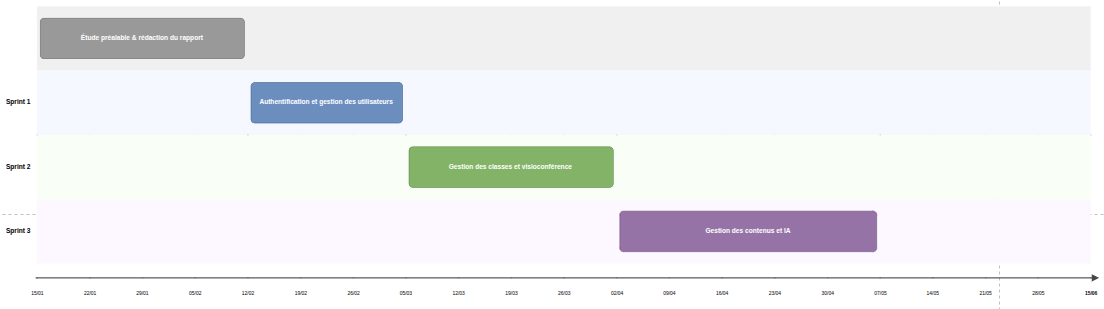
\includegraphics[width=\textwidth]{images/GANTT.png}
    \caption{Chronogramme de réalisation (Diagramme de Gantt)}
    \label{fig:gantt}
\end{figure}



% --- Section 3 : Modélisation ---
\section{Modélisation Sémantique et Comportementale}

La modélisation des besoins a pour objectif de transformer les exigences fonctionnelles en une représentation graphique claire des interactions entre les utilisateurs et le système. À cet effet, nous utilisons le \textbf{Diagramme de Cas d'Utilisation (Use Case Diagram)} issu du langage UML. 

Le diagramme présenté ci-dessous (voir Figure \ref{fig:use_case_global}) synthétise l'ensemble des interactions entre les trois acteurs du système et les fonctionnalités de la plateforme. Les trois acteurs héritent d'un acteur générique \textbf{Utilisateur} qui peut s'authentifier, gérer son profil et communiquer. Chaque acteur dispose de privilèges spécifiques :

\begin{itemize}
    \item \textbf{Administrateur :} Gère les utilisateurs (création, modification, suppression), les classes, les départements et les plannings.
    \item \textbf{Enseignant :} Gère les cours, les évaluations (manuelles ou par IA), les sessions vidéo via \textbf{Daily.co} et le suivi des présences.
    \item \textbf{Étudiant :} Consulte les cours, passe les évaluations et consulte sa progression.
\end{itemize}

\subsection{Diagramme de Cas d'Utilisation Global}

\newpage
\begin{figure}[ht!]
    \centering
    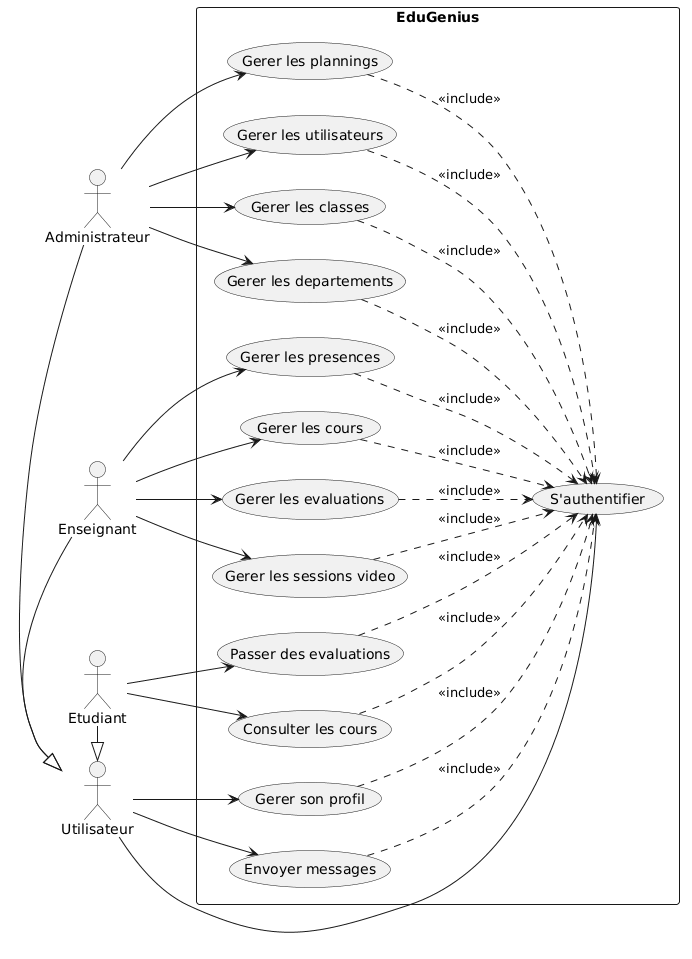
\includegraphics[width=0.85\textwidth, height=0.85\textheight, keepaspectratio]{images/use_case_global_diagram.png}
    \caption{Diagramme de cas d'utilisation global d'EduGenius}
    \label{fig:use_case_global}
\end{figure}

% --- Section 4 : Stack Technique ---
\section{Écosystème de Développement et Stack Technologique}

\subsection{Environnement de Collaboration}
Le succès du développement d'EduGenius repose sur une orchestration rigoureuse des outils de collaboration, permettant une gestion fluide du code source et du suivi de projet :

\begin{itemize}
    \item \textbf{GitHub :} Plateforme de forge logicielle utilisant Git pour le versionnement du code, facilitant le suivi des modifications et la sécurité des sources. \\ \begin{center} 
\includegraphics[width=3.5cm, height=1.2cm]{images/github_logo.png} \captionof{figure}{Logo GitHub} \end{center}
    \item \textbf{Trello :} Outil de gestion de projet basé sur la méthode Kanban, utilisé ici pour piloter le Product Backlog et l'avancement des Sprints Scrum. \\ \begin{center} 
\includegraphics[width=3.5cm, height=1.2cm]{images/trello_logo.png} \captionof{figure}{Logo Trello} \end{center}
    \item \textbf{Microsoft Teams :} Hub collaboratif utilisé pour centraliser les échanges, la documentation technique et les réunions de cadrage. \\ \begin{center} 
\includegraphics[width=3.5cm, height=1.2cm]{images/teams_logo.png} \captionof{figure}{Logo Microsoft Teams} \end{center}
\end{itemize}

\subsection{Stack Technologique : Le choix de la Performance}
L'architecture d'EduGenius repose sur une stack moderne, choisie pour sa capacité à gérer l'asynchronisme, la scalabilité et l'intégration de services temps réel :

\begin{itemize}
    \item \textbf{Next.js :} Framework full-stack basé sur React, utilisé pour le rendu hybride (SSR/SSG) et ses capacités de \textit{Server Actions}, optimisant ainsi la vitesse et le référencement \cite{nextjs_docs}. \\ \begin{center} 
\includegraphics[width=3.5cm, height=2.5cm, keepaspectratio]{images/next_logo.png} \captionof{figure}{Logo Next.js} \end{center}
    \item \textbf{Node.js \& Express :} Environnement d'exécution JavaScript côté serveur associé à un framework minimaliste pour la création d'API REST robustes et rapides \cite{learning_node}. \\ \begin{center} 
\includegraphics[width=3.5cm, height=1.2cm]{images/node_logo.png} \hspace{0.5cm} 
\includegraphics[width=3.5cm, height=1.2cm]{images/express_logo.png} \captionof{figure}{Logos Node.js et Express} \end{center}
    \item \textbf{MongoDB :} Base de données NoSQL orientée documents, offrant une grande flexibilité pour modéliser des structures de données éducatives évolutives \cite{mern_stack}. \\ \begin{center} 
\includegraphics[width=3.5cm, height=1.2cm]{images/mongodb_logo.png} \captionof{figure}{Logo MongoDB} \end{center}
    \item \textbf{AWS S3 :} Service de stockage d'objects cloud hautement disponible, utilisé pour l'hébergement sécurisé des supports de cours et fichiers multimédias. \\ \begin{center} 
\includegraphics[width=4cm, height=2cm]{images/s3_logo.png} \captionof{figure}{Logo AWS S3} \end{center}
    \item \textbf{Ollama :} Moteur d'inférence permettant l'exécution de modèles de langage (LLM) en local, garantissant la souveraineté et la confidentialité totale des données traitées \cite{generative_ai_survey}. \\ \begin{center} 
\includegraphics[width=3.5cm, height=3cm, keepaspectratio]{images/ollama_logo.png} \captionof{figure}{Logo Ollama} \end{center}
    \item \textbf{Daily.co :} API WebRTC spécialisée dans la vidéo haute définition, permettant l'intégration fluide des classes virtuelles directement dans l'interface \cite{webrtc_standard}. \\ \begin{center} 
\includegraphics[width=3.5cm, height=1.2cm]{images/daily_logo.png} \captionof{figure}{Logo Daily.co} \end{center}
    \item \textbf{Tailwind CSS :} Framework CSS utilitaire permettant une conception d'interface utilisateur rapide, moderne et entièrement responsive. \\ \begin{center} 
\includegraphics[width=3.5cm, height=2cm]{images/tailwind_logo.png} \captionof{figure}{Logo Tailwind CSS} \end{center}
    \item \textbf{Jest :} Framework de tests unitaires JavaScript, utilisé pour garantir la qualité du code et la non-régression des fonctionnalités métier par l'automatisation des tests. \\ \begin{center} 
\includegraphics[width=3.5cm, height=2cm, keepaspectratio]{images/jest.png} \captionof{figure}{Logo Jest} \end{center}
    \item \textbf{Postman :} Plateforme de collaboration pour le développement d'API, utilisée pour tester, simuler et documenter les endpoints REST du système de manière visuelle. \\ \begin{center} 
\includegraphics[width=3.5cm, height=2cm, keepaspectratio]{images/postman.png} \captionof{figure}{Logo Postman} \end{center}
    \item \textbf{Artillery :} Outil de test de charge et de performance moderne, utilisé pour simuler des flux d'utilisateurs intensifs et valider la scalabilité du système sous haute tension. \\ \begin{center} 
\includegraphics[width=4cm, height=2cm, keepaspectratio]{images/artillery_logo.png} \captionof{figure}{Logo Artillery} \end{center}
\end{itemize}

% --- Section 5 : Architecture ---
\section{Architecture Logicielle et Topologie Système}

L'architecture d'\textbf{EduGenius} a été conçue pour répondre à des impératifs de performance, de sécurité des données et de fluidité utilisateur. Elle repose sur une infrastructure hybride alliant services cloud et traitement local souverain, tout en respectant les principes de découplage de la \textit{Clean Architecture} \cite{clean_architecture}. Cette section détaille successivement l’organisation logique en couches puis la topologie matérielle et réseau.

\subsection{Architecture applicative (logique) : Modèle multi-tiers}

Le système adopte une architecture en couches (\textit{n-tier}), garantissant une séparation stricte des préoccupations (\textit{Separation of Concerns}) :

\begin{enumerate}
    \item \textbf{Couche de Présentation :} Développée avec \textbf{Next.js}, elle gère l'interface utilisateur, l'état applicatif et les interactions temps réel.
    \item \textbf{Couche Métier (Logic) :} Le serveur \textbf{Node.js} (Express) centralise la logique décisionnelle : orchestration de l'IA, gestion des sessions \textbf{Daily.co} et sécurité (JWT).
    \item \textbf{Couche d'Accès aux Données :} Interface avec \textbf{MongoDB} via l'ODM \textbf{Mongoose}, assurant la validation des schémas et l'intégrité des transactions.
\end{enumerate}

\subsection{Architecture physique (déploiement)}

La topologie de déploiement repose sur les composants suivants, interconnectés via les protocoles et flux représentés sur la figure \ref{fig:deployment_arch} :

\begin{itemize}
    \item \textbf{Clients :} Navigateurs web (desktop/mobile) communiquant en HTTPS/TLS 1.3 avec le serveur d’application.
    \item \textbf{Serveur d’application :} Instance VPS hébergeant les runtimes \textbf{Next.js} (rendu frontend) et \textbf{Express.js} (API REST). Il assure l’authentification JWT et orchestre les appels aux services externes.
    \item \textbf{Base de données :} Cluster \textbf{MongoDB Atlas} pour la persistance des utilisateurs, classes, cours, quiz et présences. La connexion s’effectue via l’ODM Mongoose.
    \item \textbf{Stockage objet :} Bucket \textbf{AWS S3} pour les fichiers volumineux (PDF, vidéos). L’accès se fait par URLs signées, soit directement par le client, soit via le backend.
    \item \textbf{Moteur IA local :} Serveur \textbf{Ollama} (modèle Gemma 3B) exécuté sur une machine dédiée, accessible via TCP/11434 en réseau interne. Toutes les données pédagogiques restent souveraines.
    \item \textbf{Service visioconférence :} \textbf{Daily.co} (cloud externe) est piloté en REST par l’application et fournit aux clients des flux WebRTC pour les classes virtuelles.
\end{itemize}

\begin{figure}[H]
    \centering
    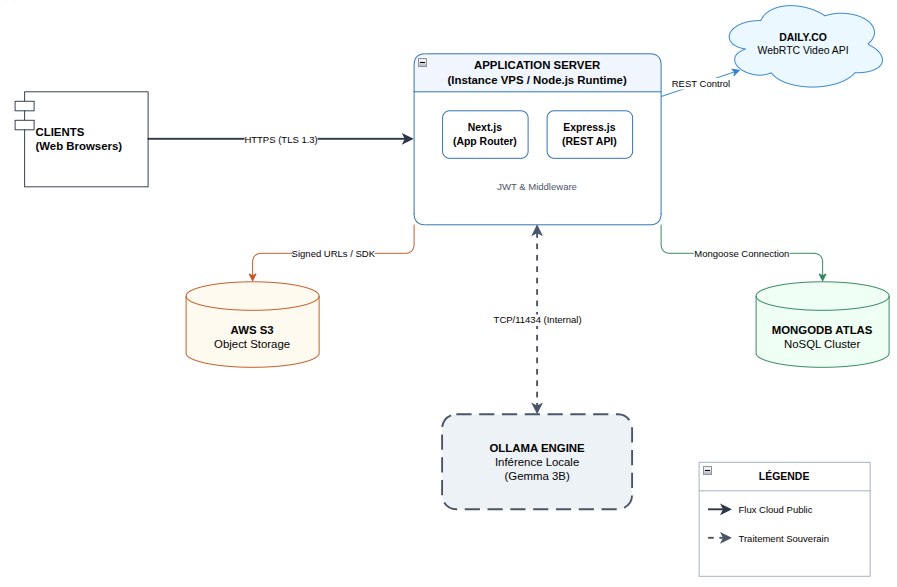
\includegraphics[width=\textwidth]{images/physical_architecture_diagram.png}
    \caption{Architecture de déploiement et flux d'infrastructure (physique)}
    \label{fig:deployment_arch}
\end{figure}

Cette infrastructure hybride garantit la scalabilité, la sécurité des données sensibles (traitement IA en local) et une expérience utilisateur fluide grâce à l’intégration native des services cloud.

% --- Conclusion du chapitre ---
\section*{Conclusion}
\addcontentsline{toc}{section}{Conclusion}

Ce chapitre a posé les bases conceptuelles et techniques du projet. L'analyse des besoins, la modélisation UML et les choix architecturaux retenus (Next.js, Express, MongoDB, Ollama, Daily.co) constituent un cadre solide pour les sprints de réalisation. Le chapitre suivant détaillera la mise en œuvre du Sprint 1, dédié à l'authentification et à la gestion des utilisateurs.